\subsection{Amministratore}

\subsubsection{Panoramica amministratore}
\begin{figure}[H]
\centering
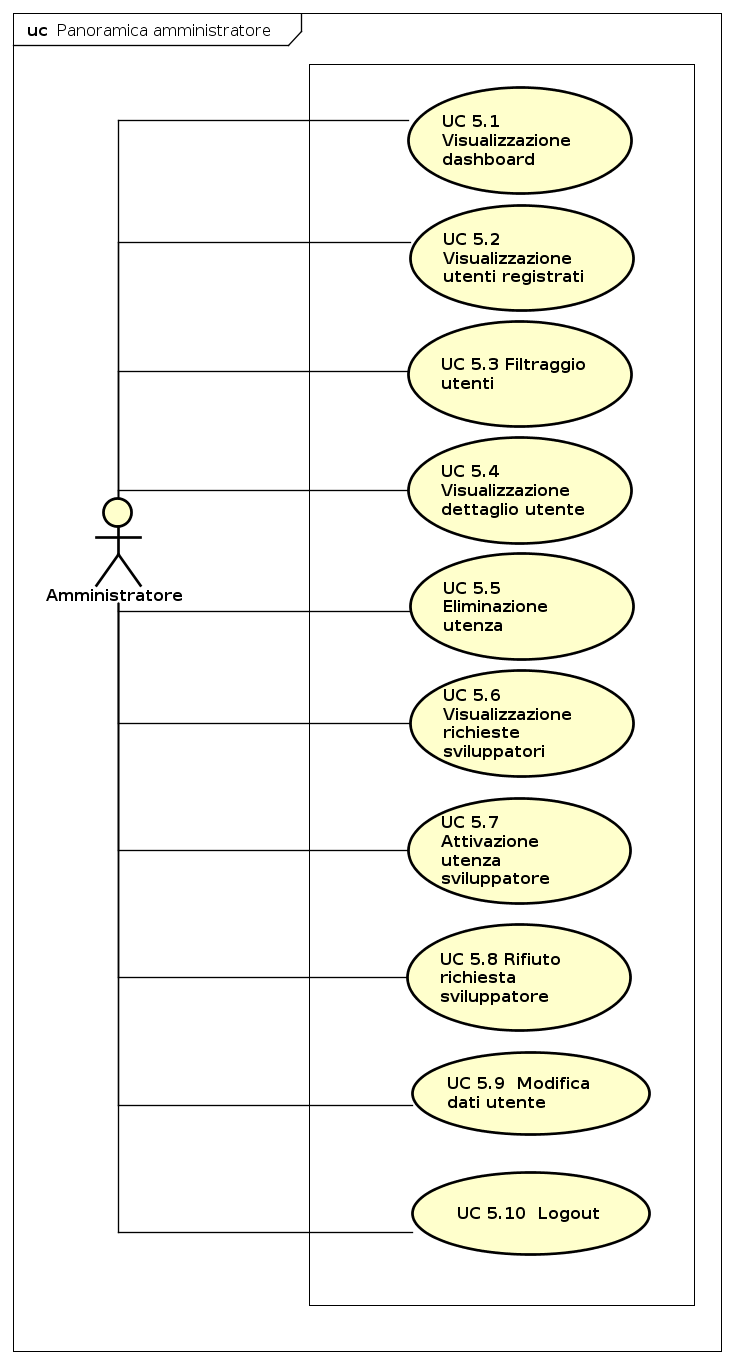
\includegraphics[width=11cm, keepaspectratio]{img/PanoramicaAmministratore.png} 
\caption{Panoramica amministratore}
\end{figure}


\subsubsection{UC 5.1 - Visualizzazione dashboard}

\begin{itemize}
\item \textbf{Attore}: Amministratore; 
\item \textbf{Descrizione}: l'amministratore visualizza la propria dashboard;
\item \textbf{Precondizione}: l'amministratore si è autenticato;
\item \textbf{Postcondizione}: l'amministratore visualizza la sua dashboard e può accedere alle seguenti funzionalità: visualizzazione utenti registrati con relativo filtraggio dati, visualizzazione richieste da parte degli sviluppatori che intendono accedere ai dati del sistema ed accedere alla pagina di modifica dei dati personali;
\item \textbf{Flusso degli eventi}: l'amministratore accede alla propria dashboard personale.
\end{itemize}

\subsubsection{UC 5.2 - Visualizzazione utenti registrati}

\begin{itemize}
\item \textbf{Attore}: Amministratore;
\item \textbf{Descrizione}: l'amministratore visualizza l'elenco degli utenti registrati nel sistema;
\item \textbf{Precondizione}: l'amministratore si è autenticato;
\item \textbf{Postcondizione}: l'amministratore visualizza tutti gli utenti registrati nel sistema;
\item \textbf{Flusso degli eventi}: l'amministratore accede alla propria dashboard e visualizza l'elenco degli utenti registrati nel sistema.
\end{itemize}

\subsubsection{UC 5.3 - Filtraggio utenti}
\begin{itemize}
\item \textbf{Attore}: Amministratore;
\item \textbf{Descrizione}: l'amministratore può filtrare gli utenti;
\item \textbf{Precondizione}: l'amministratore si è autenticato;
\item \textbf{Postcondizione}: l'amministratore visualizza la lista degli utenti in base ai filtri applicati;
\item \textbf{Flusso degli eventi}: l'amministratore visualizza elenco utenti ed ha la possibilità di filtrate.
\end{itemize}
\subsubsection{UC 5.4 - Visualizzazione dettaglio utente}
\begin{itemize}
\item \textbf{Attore}: Amministratore;
\item \textbf{Descrizione}: l'amministratore visualizza in dettaglio un utente specifico visualizzandone tutti i dati inseriti da quest'ultimo in fase di registrazione;
\item \textbf{Precondizione}: l'amministratore visualizza la lista degli utenti;
\item \textbf{Postcondizione}: l'amministratore visualizza le informazioni personali dell'utente;
\item \textbf{Flusso degli eventi}: l'amministratore visualizza l'elenco utenti ed ha la possibilità di visualizzare un utente nel dettaglio.
\end{itemize}


\subsubsection{UC 5.5 - Eliminazione utenza}
\begin{itemize}
\item \textbf{Attore}: Amministratore;
\item \textbf{Descrizione}: l'amministratore elimina un'utenza dal sistema;
\item \textbf{Precondizione}: l'amministratore visualizza l'elenco degli utenti registrati nel sistema;
\item \textbf{Postcondizione}: l'amministratore ha eliminato l'utenza dal sistema;
\item \textbf{Flusso degli eventi}: l'amministratore visualizza elenco utenti ed ha la possibilità di eliminare un'utenza.
\end{itemize}


\subsubsection{UC 5.6 - Visualizzazione richieste sviluppatori}
\begin{itemize}
\item \textbf{Attore}: Amministratore;
\item \textbf{Descrizione}: l'amministratore visualizza le richieste degli utenti;
\item \textbf{Precondizione}: l'amministratore si trova nella dashboard;
\item \textbf{Postcondizione}: l'amministratore visualizza l'elenco delle richieste in sospeso;
\item \textbf{Flusso degli eventi}:  l'amministratore visualizza tutte le richieste degli utenti che vogliono ottenere il ruolo di sviluppatore nel sistema.
\end{itemize}

\subsubsection{UC 5.7 - Attivazione utenza sviluppatore}
\begin{itemize}
\item \textbf{Attore}: Amministratore;
\item \textbf{Descrizione}: l'amministratore può attivare utenza in sospeso;
\item \textbf{Precondizione}: l'amministratore visualizza la lista delle richieste in sospeso degli sviluppatori;
\item \textbf{Postcondizione}: l'utenza dello sviluppatore è stata attivata e lo sviluppatore può quindi accedere al sistema;
\item \textbf{Flusso degli eventi}: l'amministratore attiva un utente che ha fatto richiesta come sviluppatore.
\end{itemize}

\subsubsection{UC 5.8 - Rifiuto richiesta sviluppatore}
\begin{itemize}
\item \textbf{Attore}: Amministratore;
\item \textbf{Descrizione}: l'amministratore può rifiutare utenza in sospeso;
\item \textbf{Precondizione}: l'amministratore visualizza la lista delle richieste in sospeso degli sviluppatori;
\item \textbf{Postcondizione}: l'utenza dello sviluppatore è stata rifiutata;
\item \textbf{Flusso degli eventi}: l'amministratore rifiuta la richiesta avanzata da uno sviluppatore.
\end{itemize}

\subsubsection{Panoramica modifica dati utente}
\begin{figure}[H]
	\centering
	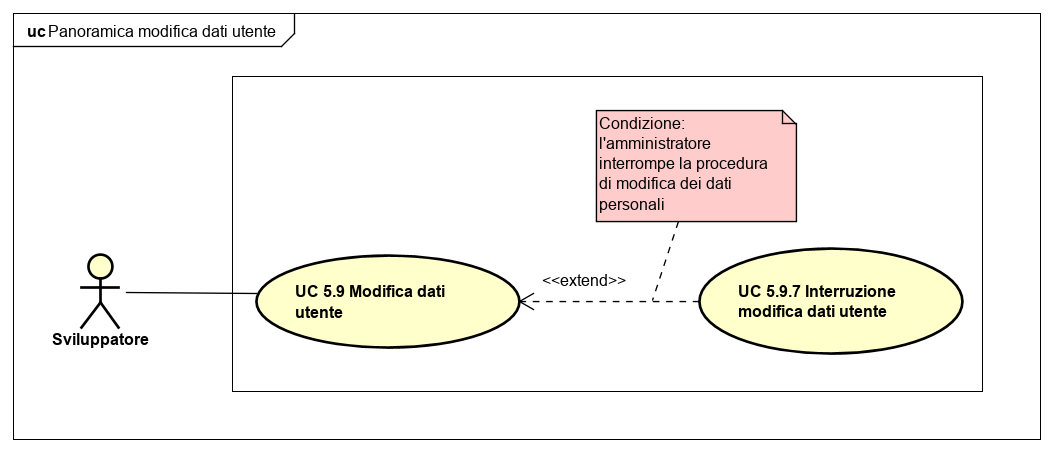
\includegraphics[width=12cm, keepaspectratio]{img/panmod59.png} 
	\caption{Caso d'uso UC 5.9:Panoramica modifica dati utente per Ammininistratore}\label{fig:Panoramica modifica dati utente per Ammininistratore}
\end{figure}

\subsubsection{UC 5.9 - Modifica dati utente}
\begin{figure}[H]
	\centering
	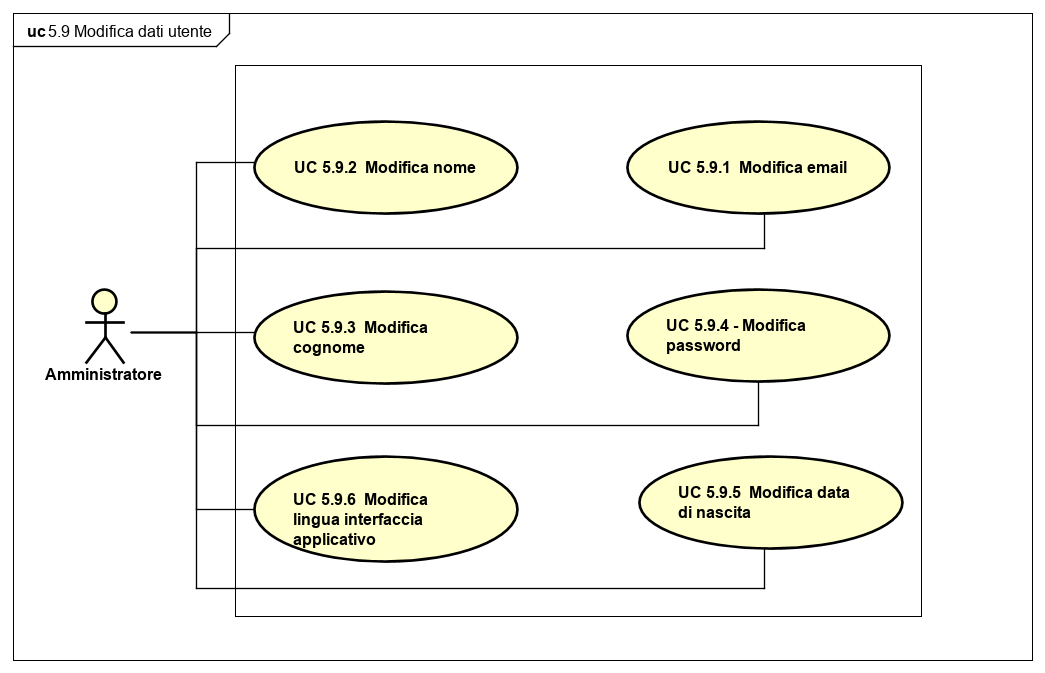
\includegraphics[width=12cm, keepaspectratio]{img/UC59.png} 
	\caption{Caso d'uso UC 5.9:  Modifica dati utente per Ammininistratore}\label{fig:411}
\end{figure}
\begin{itemize}
	\item[•]\textbf{Attori}: Amministratore;
	\item[•]\textbf{Descrizione}: l'amministratore modifica i propri dati personali, cioè tutti i dati personali inseriti in fase di registrazione;
	\item[•]\textbf{Precondizione}: l'amministratore visualizza la propria dashboard;
	\item[•]\textbf{Postcondizione}: l'amministratore ha modificato uno o più dati personali; 
	\item[•]\textbf{Flusso degli eventi}: 
	\begin{enumerate}
		\item Selezione procedura modifica dati personali;
		\item UC 5.9.1 - Modifica email; 
		\item UC 5.9.2 - Modifica nome;
		\item UC 5.9.3 - Modifica cognome;
		\item UC 5.9.4 - Modifica password;
		\item UC 5.9.5 - Modifica data di nascita;
		\item UC 5.9.6 - Modifica lingua interfaccia applicativo;
		\item Conferma modifica dati.
	\end{enumerate}
	\item[•] \textbf{Estensioni}:	
	\begin{enumerate}
		\item UC 5.9.7 - Interruzione modifica dati utente.
	\end{enumerate}
\end{itemize}
\subsubsection{UC 5.9.1 - Modifica email}
\begin{itemize}
	\item[•]\textbf{Attori}: Amministratore;
	\item[•]\textbf{Descrizione}: l'amministratore modifica la propria email;
	\item[•]\textbf{Precondizione}: l'amministratore sta modificando i propri dati personali;
	\item[•]\textbf{Postcondizione}: l'amministratore ha modificato la propria email; 
	\item[•]\textbf{Flusso degli eventi}: 
	\begin{enumerate}
		\item Selezione campo email;
		\item Modifica la stringa che rappresenta la propria email.
	\end{enumerate}
\end{itemize}
\subsubsection{UC 5.9.2 - Modifica nome}
\begin{itemize}
	\item[•]\textbf{Attori}: Amministratore;
	\item[•]\textbf{Descrizione}: l'amministratore modifica il proprio nome;
	\item[•]\textbf{Precondizione}: l'amministratore sta modificando i propri dati personali;
	\item[•]\textbf{Postcondizione}: l'amministratore ha modificato il proprio nome; 
	\item[•]\textbf{Flusso degli eventi}: 
	\begin{enumerate}
		\item Selezione campo nome;
		\item Modifica la stringa che rappresenta il nome.
	\end{enumerate}
\end{itemize}
\subsubsection{UC 5.9.3 - Modifica cognome}
\begin{itemize}
	\item[•]\textbf{Attori}: Amministratore;
	\item[•]\textbf{Descrizione}: l'amministratore modifica il proprio cognome;
	\item[•]\textbf{Precondizione}: l'amministratore sta modificando i propri dati personali;
	\item[•]\textbf{Postcondizione}: l'amministratore ha modificato il proprio cognome; 
	\item[•]\textbf{Flusso degli eventi}: 
	\begin{enumerate}
		\item Selezione campo cognome;
		\item Modifica la stringa che rappresenta il cognome.
	\end{enumerate}
\end{itemize}
\subsubsection{UC 5.9.4 - Modifica password}
\begin{figure}[H]
	\centering
	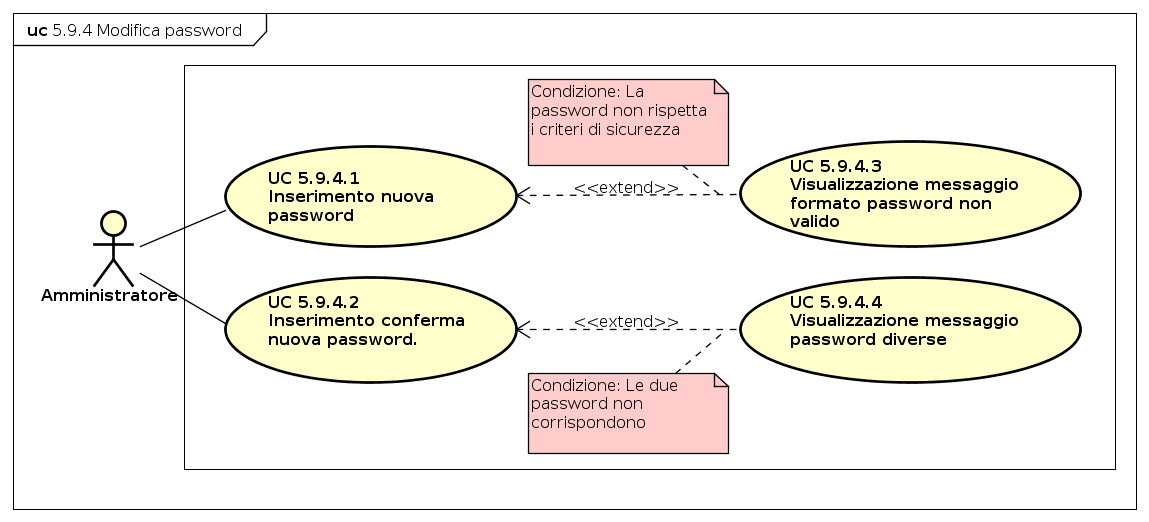
\includegraphics[width=15cm, keepaspectratio]{img/UC594.png} 
	\caption{Caso d'uso UC 5.9.4, modifica password per Amministratore}
\end{figure}
\begin{itemize}
	\item[•]\textbf{Attori}: Amministratore;
	\item[•]\textbf{Descrizione}: l'amministratore modifica il proprio cognome;
	\item[•]\textbf{Precondizione}: l'amministratore sta modificando i propri dati personali;
	\item[•]\textbf{Postcondizione}: l'amministratore ha modificato il proprio cognome; 
	\item[•]\textbf{Flusso degli eventi}: 
	\begin{enumerate}
		\item UC 5.9.4.1 - Inserimento nuova password;
		\item UC 5.9.4.2 - Inserimento conferma nuova password.
	\end{enumerate}
\end{itemize}

\subsubsection{UC 5.9.4.1 - Inserimento nuova password}
\begin{itemize}
	\item[•]\textbf{Attori}: Amministratore;
	\item[•]\textbf{Descrizione}: l'amministratore inserisce la nuova password;
	\item[•]\textbf{Precondizione}: l'amministratore sta modificando i propri dati personali;
	\item[•]\textbf{Postcondizione}: l'amministratore ha inserito il valore della nuova password; 
	\item[•]\textbf{Flusso degli eventi}: 
	\begin{enumerate}
		\item Selezione campo dati relativo alla nuova password;
		\item Inserimento stringa rappresentante la password.
	\end{enumerate}
	\item[•]\textbf{Estensioni}:
	\begin{enumerate}
		\item UC 5.9.4.3 - Visualizzazione messaggio formato password non valido.
	\end{enumerate}
\end{itemize}

\subsubsection{UC 5.9.4.2 - Inserimento conferma nuova password}
\begin{itemize}
	\item[•]\textbf{Attori}: Amministratore;
	\item[•]\textbf{Descrizione}: l'amministratore inserisce conferma la nuova password, reinserendola nell'apposito campo;
	\item[•]\textbf{Precondizione}: l'amministratore sta modificando i propri dati personali;
	\item[•]\textbf{Postcondizione}: l'amministratore ha inserito il valore del campo conferma nuova password; 
	\item[•]\textbf{Flusso degli eventi}: 
	\begin{enumerate}
		\item Selezione campo dati relativo alla conferma nuova password;
		\item Inserimento stringa rappresentante la password.
	\end{enumerate}
	\item[•]\textbf{Estensioni}:
	\begin{enumerate}
		\item UC 5.9.4.4 - Visualizzazione messaggio password diverse.
	\end{enumerate}
\end{itemize}

\subsubsection{UC 5.9.4.3 - Visualizzazione messaggio formato password non valido}
\begin{itemize}
	\item[•]\textbf{Attori}: Amministratore;
	\item[•]\textbf{Descrizione}: l'amministratore ha inserito una password con un formato non valido;
	\item[•]\textbf{Precondizione}: l'amministratore sta modificando i propri dati personali;
	\item[•]\textbf{Postcondizione}: l'amministratore visualizza un messaggio di errore relativo all'inserimento di una password che non rispetta un formato valido; 
	\item[•]\textbf{Flusso degli eventi}: l'amministratore ha inserito una password che non rispetta i criteri accettati dal sistema, pertanto riceve un messaggio che indica la presenza di un formato non adatto.
\end{itemize}

\subsubsection{UC 5.9.4.4 - Visualizzazione messaggio password diverse}
\begin{itemize}
	\item[•]\textbf{Attori}: Amministratore;
	\item[•]\textbf{Descrizione}: l'amministratore ha inserito un valore di conferma password che non corrisponde al valore della nuova password inserita precedentemente, pertanto visualizza un messaggio che indica che le due password non corrispondono;
	\item[•]\textbf{Precondizione}: l'amministratore ha inserito il valore del campo conferma nuova password;
	\item[•]\textbf{Postcondizione}: l'amministratore visualizza un messaggio di errore relativo all'inserimento di una password che non combacia con quella inserita nel campo nuova password; 
	\item[•]\textbf{Flusso degli eventi}: l'amministratore ha inserito una password che non combacia con quella inserita nel campo nuova password, pertanto riceve un messaggio che indica la presenza di tale difformità.
\end{itemize}

\subsubsection{UC 5.9.5 - Modifica data di nascita}
\begin{itemize}
	\item[•]\textbf{Attori}: Amministratore;
	\item[•]\textbf{Descrizione}: l'amministratore modifica il proprio cognome;
	\item[•]\textbf{Precondizione}: l'amministratore sta modificando i propri dati personali;
	\item[•]\textbf{Postcondizione}: l'amministratore ha modificato il proprio cognome; 
	\item[•]\textbf{Flusso degli eventi}: 
	\begin{enumerate}
		\item Selezione campo data di nascita;
		\item Modifica la stringa che rappresenta la data di nascita, inserendo il valore corretto.
	\end{enumerate}
\end{itemize}
\subsubsection{UC 5.9.6 - Modifica lingua interfaccia applicativo}
\begin{itemize}
	\item[•]\textbf{Attori}: Amministratore;
	\item[•]\textbf{Descrizione}: l'amministratore modifica la lingua dell'applicativo;
	\item[•]\textbf{Precondizione}: l'amministratore sta modificando i propri dati personali;
	\item[•]\textbf{Postcondizione}: l'amministratore ha modificato la lingua dell'applicativo; 
	\item[•]\textbf{Flusso degli eventi}: 
	\begin{enumerate}
		\item Selezione campo dati lingua applicativo;
		\item Selezione da un elenco predefinito la lingua dell'applicativo desiderata.
	\end{enumerate}
\end{itemize}

\subsubsection{UC 5.9.7 - Interruzione modifica dati utente}
\begin{itemize}
	\item[•]\textbf{Attori}: Amministratore;
	\item[•]\textbf{Descrizione}: l'amministratore interrompe la procedura di modifica dei dati utente;
	\item[•]\textbf{Precondizione}: l'amministratore sta modificando i propri dati;
	\item[•]\textbf{Postcondizione}: l'amministratore abbandona la procedura e nessuna modifica è stata effettuata nel sistema; 
	\item[•]\textbf{Flusso degli eventi}: l'amministratore abbandona la pagina di modifica dei dati e viene reindirizzato alla dashboard.
\end{itemize}


\subsubsection{UC 5.10 - Logout}
\begin{itemize}
    \item[•] \textbf{Attori}: Amministratore;
    \item[•] \textbf{Descrizione}:  l'amministratore effettua il logout dal sistema;
    \item[•] \textbf{Precondizione}: l'amministratore si è autenticato;
    \item[•] \textbf{Postcondizione}: l’amministratore effettua il logout dal sistema e viene reindirizzato alla pagina di login;
    \item[•] \textbf{Flusso degli eventi}: l’amministratore seleziona il bottone di logout e esce dalla sessione.
\end{itemize}



